% !TeX encoding = UTF-8
% !TEX root = ./presentation.tex
\section{HLS}

\section{FPGA}
   
   \begin{frame}{Tecnologia dos FPGA} \vspace{-1em}
      \textbf{Vários módulos lógicos programáveis} relativamente \textbf{pequenos} e independentes, interconectados.
      
      \begin{itemize}
         \item A maioria dos FPGAs utilizam \textit{look-up table} (LUT) para criar as funções lógicas desejadas.
         \begin{itemize} 
            \setlength{\itemsep}{1.5em}
            \item Uma LUT funciona como uma tabela-verdade, ou seja, registradores programáveis. 
            \item Cada módulo lida com até quatro ou cinco variáveis de entrada;
            \item A saída é programada para criar a função combinacional armazenando valores verdadeiros e falsos adequado a cada combinação de entrada;
            \item Eles não são associados a nenhum pino de entrada e saída (I/O, do inglês \textit{Input and Output}). 
         \end{itemize}
         
      \end{itemize}
      \pdfnote{pequenos pra criar funções +}
   \end{frame}
   
   
   \begin{frame}{Tecnologia dos FPGA} \vspace{-1em}
      Vários módulos lógicos programáveis relativamente \textbf{pequenos} e \textbf{independentes}, \textbf{interconectados}.
      
      \begin{itemize}
      \setlength{\itemsep}{1.2em}
      
      \item Os recursos de roteamento de sinal programável dentro do chip
      \begin{itemize}
         \item Os atrasos de sinal em um projeto dependem do roteamento real de sinal selecionado pelo \software\ de programação. 
      \end{itemize}
      
      \item Pinos de I/O são conectados ao bloco programável de entrada e saída que, por sua vez, é conectado aos módulos lógicos com linhas de roteamento selecionadas.
      \bigskip
      \item Assim, FPGAs são chips que podem ser programados instantaneamente para funções de qualquer circuito digital \cite{Choi2016}.   
      \end{itemize}
      \pdfnote{pequenos pra criar funções +}
   \end{frame}


\begin{frame}{FPGA}{Sua Tecnologia \cite{tocci2003sistemas}} \vspace{-1em}
\begin{itemize}
\setlength{\itemsep}{0.8em}          
\item Utilizar tecnologia CMOS
\begin{itemize}
   \item \textbf{Consumo de energia} é relativamente \textbf{baixo};
   \item \textbf{Pode-se confeccionar} em nível de tensão elétrica, frequências e cargas para os sinais de I/O. 
\end{itemize}

\item Existem diferentes FPGAs
\begin{itemize}
   \item Tamanho e velocidades diferentes;
\end{itemize}

\item Mas, como pode ser configurado para um número infinito de projetos
\begin{itemize}
   \item \textbf{Não é possível afirmar o montante de dissipação de energia} para um dispositivo FPGA de modo geral
\end{itemize}

\end{itemize}
\pdfnote{Quartus estima ouso de energia. }
\pdfnote{Voltado para indústria e até mesmo educação}
\end{frame}

\begin{frame}{FPGA}{Vantagens \cite{tocci2003sistemas, Plessl2003}}
\begin{itemize} \setlength{\itemsep}{1.2em}
\item - Ao invés de diversos circuitos individuais;
\item + Programar a mesma funcionalidade destes.
\bigskip
\item + Maior confiabilidade;
\item + Menor:
\begin{itemize}
\item Espaço ocupado na placa;
\item Consumo de energia;
\item Complexidade de desenvolvimento; e, geralmente, \item Menor custo de fabricação.
\end{itemize}
\end{itemize}
\end{frame}


\section{Wearable}

\begin{frame}{Características de um \Wearable} \vspace{-1em}
\begin{itemize}
   \setlength{\itemsep}{1.5em}
   \item Já \cite{Jozwiak2017} caracteriza como um sistema \textit{cyber}-físico\footnote{Sendo \textit{cyber-} uma combinação dos termos `computador', `rede de computadores' ou `realidade virtual' com um segundo termo, no caso o `físico' oriundo de circuitos.} móvel autônomo.
   
   \item Podem ser utilizados para aplicações de consumidores, extensões ou reposição de capacidades humanas, ou industriais
   
   \item Representam uma grande parte da heterogeneidade de sistemas embarcados, 
   \begin{itemize}
      \setlength{\itemsep}{1.0em}
      \item Desde um dispositivo inteligente integrado à roupa, focado no campo de computação \textit{mobile} pessoal, até indústrias como dispositivos de segurança. % \citep{Jozwiak2017}.
      \item Podem trabalhar de forma colaborativa com \textit{smartphones}, redes e outros sistemas criando um sistema mais complexo.
   \end{itemize}
\end{itemize}
\end{frame}


\begin{frame}{Características de um \Wearable} \vspace{-1em}
Segundo \cite{VanLaerhoven2002}, a distribuição de elementos computacionais, sensores, em objetos mundanos em nosso cotidiano se adéqua à computação ubíqua. 
\begin{itemize}
\setlength{\itemsep}{1.5em}
\item Na qual computação \wearable\ também não foge deste ramo
\begin{itemize}
   \item Superfícies de roupas são uma plataforma de suporte ideal para uma grande quantidade de sensores.
\end{itemize}
\item A restrição de tamanho relaciona-se com a própria qualidade do equipamento
\begin{itemize}
   \item Levando muitos atuadores e sensores a serem simplistas.
\end{itemize}
\end{itemize}
\end{frame}

\section{Trabalhos Relacionados}

\begin{comment}
\begin{frame} \vspace{-1em}
\begin{columns}
\begin{column}{0.4\textwidth}
\begin{block}{Definição Introdutória Particionamento \cite{Arato2005}}
Problema de otimização na qual utiliza-se métodos para auxiliar na decisão de cada componente do \design\ referencial. 
\end{block}
\end{column}
\begin{column}{0.6\textwidth}

\begin{figure}[h] \centering
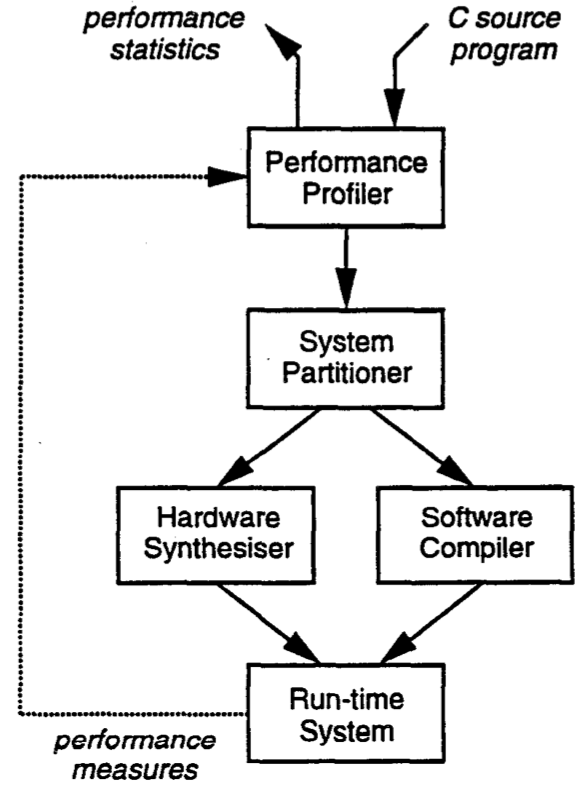
\includegraphics[width=0.8\textwidth]{img/rt-edwards_method.png}
\caption{Metodologia de \codesign. Fonte: \cite{Edwards1994}.}
\label{fig:tr-edwards_method}
\end{figure}
\end{column}
\end{columns}   

\pdfinfo{Tanto processos manuais, exatos ou heurísticos.}
\end{frame}

\begin{frame}{Pioneiro: \cite{Edwards1994}} \vspace{-1em}
\begin{itemize}
\setlength{\itemsep}{1.3em}
\item Utilizam do particionamento para aprimorar a performance do seu \software. 
\item Realiza-se a tentativa de tratar regiões críticas da aplicação 
\begin{itemize}
\item A solução em \software\ não pode chegar à restrições de performance requeridas;
\end{itemize}

\item Apresenta-se uma metodologia para desenvolvimento \codesign.
\begin{itemize}
\setlength{\itemsep}{1.0em}
\item Consiste na construção do código da aplicação em \textit{C} e sua análise;
\item Regiões críticas são identificadas e particionadas. 
\end{itemize}

\item Feito isso, realizar-se mensurações
\begin{itemize}
\item  Um novo particionamento é feito.
\end{itemize}

\item Utiliza-se de um FPGA.
\end{itemize}
\end{frame}

\begin{frame}{Trabalhos com Foco em Otimizações} \vspace{-1em}
\begin{itemize}
\setlength{\itemsep}{1.2em}
\item \cite{Stitt2003} pioneiro no método de otimização \textbf{dinâmico}.

\item Processos:
\begin{enumerate}
\setlength{\itemsep}{0.8em}
\item Detecta a região de mais executada e;
\item Reimplementa-a em \hardware\ de FPGA.
\end{enumerate}

\item Afirmam isso vantagens comparado com abordagens tradicionais manuais.

\item Como Stitt, outros propuseram algoritmos \textbf{exatos} baseados em estratégias:
\begin{itemize}
\setlength{\itemsep}{0.8em}
\item \textit{Branch-and-Bound} \cite{Jigang2004, Mann2007, Strachacki2008};
\item Programação dinâmica \cite{Madsen1997, Wu2006} e;
\item Programação Linear inteira \cite{Niemann1997}.
\end{itemize}
\end{itemize}
\end{frame}

\begin{frame}{Trabalhos com Foco em Otimizações} \vspace{-1em}
\begin{itemize}
\setlength{\itemsep}{1.8em}
\item \cite{Nematbakhsh_theeffect} exame da relação entre o \textit{footprint} do FPGA e o \speedup\ do \software.
\begin{itemize}
\item FPGA utilizado na implementação de \textit{loops} e sub-rotinas críticas.
\end{itemize}

\item Abordagem direta utilizando ferramentas comerciais como \textit{Synopys' Nimble Compiler} e \textit{Proceler} para a facilitação do processo.

\item \cite{Yan2017} parte da otimização \textit{position disturbed particle swarm} com otimização invasiva de \textit{weed} como o método de particionamento \hs.
\end{itemize}
\end{frame}

\begin{frame}{\cite{Wang2016}} \vspace{-1em}
\begin{itemize}
\setlength{\itemsep}{1.7em}
\item ``Particionamento depende da exploração de caracterização, estimação e \design\ espacial das métricas de custo e performance sistêmica.''
\begin{itemize}
\item Citam o \codesign\ é tão complexo que a simplificação do particionamento só para duas partes não é suficiente para a representação do problema como um todo. 
\end{itemize}

\item Incluem parâmetros chave de \design\ e uso de recursos que deveriam ser incorporados à modelagem do sistema
\begin{itemize}
\item Considera a modelagem de incerteza para particionamento de sistemas com um conjunto melhorado de parâmetros para compartilhamento de recursos \hs.
\end{itemize}

\end{itemize}
\end{frame}

\begin{frame}{\cite{Wang2016}} \vspace{-1em}
\begin{itemize}
\item Esse terceiro item a ser considerado ao problema de particionamento podem ser definidos em três tipos, sendo esses:
\begin{enumerate}
\setlength{\itemsep}{1.5em}
\item \textbf{Conjunto de recursos necessários para particionar uma dada tarefa:} sendo esses RAM, ROM, DPS, blocos IP do inglês, \textit{intelectual propriety}, entre outros; 
\item \textbf{Parâmetros de configurações que provê diferentes \textit{trade-off} entre recursos e performances:} exemplo circuitos de multiplicações sintetizados ou não;
\item \textbf{Dificuldade da mensura de desempenho e impacto no uso de recursos em várias configurações de partição com precisão precisando ter em mente a partição com a natureza incerta\footnote{Teoria da incerteza: Matemática axiomática para modelagem de graus de crença.} dessas estimativas não precisas.}
\end{enumerate}
\end{itemize}
\end{frame}

%\frame{\centering \bf \Huge \color{beamerCinza} Sistemas Embarcados}   

\begin{frame}{Embarcados} \vspace{-1em}
\begin{itemize}
\setlength{\itemsep}{1.8em}
\item SE é amplamente pesquisado desde 90 \cite{Ernst1993, Gupta1995, Hardt1995, Gajski1994, Bolsens1997}.

\item \cite{Mei2000} Descreve um particionamento além de uma abordagem de escalonamento para DRESs\footnote{Do inglês \textit{dynamically reconfigurable embedded systems}.}
\begin{itemize}
\item Para o escalonamento, \cite{Mei2000} Algoritmo Genético.
\end{itemize}

\item Contribuições
\begin{itemize}
\setlength{\itemsep}{1.0em}
\item Análise de tempo de configuração e;
\item Análise do tempo de reconfiguração parcial do FPGA.
\end{itemize}

\end{itemize}
\pdfnote{Embedded}
\pdfnote{reconfiguração parcial -> escalonamento p. de alocação restrita.}
\end{frame}

\begin{frame}{\cite{Arato2003}} \vspace{-1em}
\begin{itemize}
\setlength{\itemsep}{1.8em}
\item Descreve versões diferentes do particionamento
\begin{itemize}
\setlength{\itemsep}{1.0em}
\item Sistemas de tempo-real e custo restringido respectivamente;
\item Fornece análise matemática formal do problema, provando que é $ \mathcal{NP} $-difícil.
\end{itemize} 

\item Utiliza 
\begin{itemize}
\setlength{\itemsep}{1.0em}
\item Programação linear inteira resolvendo de forma otimizada, e;
\item Outra utilizando GA com soluções próximas ao ótimo global.
\end{itemize}
\end{itemize}
\end{frame}

\begin{frame}{\cite{Mann2007}} \vspace{-1em}
\begin{itemize}
\setlength{\itemsep}{1.2em}
\item Descrevem uma primeira tentativa para um algoritmo exato, não heurístico, para o problema de particionamento. 

\item Implementa-se a estratégia \textit{branch-and-bound} como um \textit{framework}, permitindo o incremento de outros algoritmos. 

\item Realizaram investigações para incrementar a eficiência do algoritmo com as técnicas:
\begin{itemize}
\item \textit{Lower bounds based on LP-relaxation}, uma mecânica de inferência customizada, condições não-triviais necessárias baseadas num algoritmo \textit{minimum-cut}, e diferentes heurísticas com passos pré-otimizados. 
\end{itemize}

\item Demonstram que podem resolver problemas complexos em tempo razoável. 
\begin{itemize}
\item O resultado é em entorno de dez minutos mais rápido que algoritmos exatos anteriores baseados em programação linear inteira para os testes realizados.
\end{itemize}
\end{itemize}
\pdfnote{Prox slide: pesq mais recentes}
\end{frame}

\begin{frame}{\cite{Hassine2017}} \vspace{-1em}
\begin{itemize}
\setlength{\itemsep}{1.5em}
\item Aplicou otimizações sobre o tempo de execução e gasto energético.

\item O algoritmo proposto destina-se a alcançar um particionamento de grafos à procurar o melhor conjunto da relação energia e tempo de execução.

\item Comparou-se com \textit{Simulated Annealing}, Busca Tabu e Genético
\begin{itemize}
\item Mostra-se mais adequado para aplicações em \cores\ de sistemas embarcados que necessitam do equilíbrio no \textit{tradeoff} de sistemas embarcados.
\end{itemize}

\end{itemize}
\end{frame}

\begin{frame}{\cite{Trindade2016}} \vspace{-1em}
\begin{itemize}
\setlength{\itemsep}{1.8em}
\item Utiliza do GA para solucionar o problema.

\item Propõe novas abordagens usando técnicas de verificação baseadas nas teorias de módulo de satisfação (SMT, do inglês \textit{satisfiability modulo theories}). 

\item Apresentam um exemplo de particionamento, modelam e solucionam-o usando três diferentes técnicas
\begin{itemize}
\setlength{\itemsep}{1.0em}
\item A ideia principal é aplicar o método de verificação SMT ao particionamento, e;
\item Comparar os resultados com otimizações tradicionais como ILP e GA.
\end{itemize}

\end{itemize}
\end{frame}


\begin{frame}{\cite{Jozwiak2017}} \vspace{-1em}
\begin{itemize}
\setlength{\itemsep}{0.7em}
\item Seu \textit{survey} considera os aspectos de uma aplicação embutida
\begin{itemize}
\item Tecnologias de \design\ com foco sistemas móveis modernos e \wearables.
\end{itemize}

\item Cita-se dois paradigmas de desen. para SE sobre sistema de multi-processadores heterogêneos. O paradigma de sistemas 
\begin{itemize} \setlength{\itemsep}{0.5em}
\item \textbf{\textit{Life-inspired}:} 
\begin{itemize}
\item Especifica princípios, características e organização funcional e estrutural de SE com analogia à vida de um organismo inteligente;
\item Soluções de mecanismos e arquiteturas de sistemas para sua implementação. 
\end{itemize}

\item \textbf{\textit{Quality-driven}:} 
\begin{itemize}
\item Solução para o \design\ de disp. que necessitam de exigências de \textit{real-time}, baixo consumo de energia, entre outros; 
\item Dessa forma, especifica-se qual a nova qualidade do sistema a ser requeria e como esta meta é obtida. 
\item ``Define-se \textit{qualidade} de uma solução sistêmica proposta como o \textit{total de sua eficácia}\footnote{Grau em que uma solução atinge seus objetivos.} \textbf{e} \textit{eficiência\footnote{Grau em que uma solução usa recursos para realizar seus objetivos.} na resolução do problema real}''.
\end{itemize}
\end{itemize}

\end{itemize}
\pdfnote{ORIENTADO PELA QUALIDADE}
\pdfnote{juntas determinam o grau de EXCELÊNCIA}

\end{frame}


\begin{frame}{\cite{Jozwiak2017}} 

\begin{block}{Entretanto, descreveram ao final que \cite{Jozwiak2017}}
``Enquanto \designers\ aprenderam bastante na \textbf{construção} de plataformas de \hardware\ heterogêneos altamente paralelos, métodos e ferramentas automatizadas para a sua programação e o paralelismo do algoritmo, bem como o \codesign\ coerente da arquitetura \hs\ \textbf{ainda estão atrasados perante à tecnologia}''.
\end{block}
\end{frame}


\begin{frame}{\Wearable e FPGA}
\begin{itemize}
\setlength{\itemsep}{2em}
\item \cite{Plessl2003, Ahola2007, Abdelhedi2016, Narumi2016, Lee2015} que relacionam FPGAs com aplicação \wearable.

\item Entretanto, nenhum menciona análise metodológica do problema de particionamento \hs\ para \design\ de sistemas computacionais \wearables.
\end{itemize}
\end{frame}

\end{comment}



\section{Met1}


\begin{frame}{Grafo de Controle de Fluxo (GCF)}
\begin{itemize}
   \setlength{\itemsep}{1.6em}
   \item A decomposição de um DRS pode gerar dois componentes:
   \begin{itemize}
      \item Porção a ser realizada em \hardware\ e outra executada em \software;
   \end{itemize}
   
   \item Essa decisão de divisão é chamada de problema de particionamento.
   
   \item Para sistemas baseados em Plataformas FPGA, particionamento é um sub-problema de um problema mais geral localizado no \codesign, onde refere-se ao \design\ cooperativo.
\end{itemize}
\end{frame}

\begin{frame}

\begin{equation}
\gamma =
\frac{
   \text{\textit{hardware speed}}
}{
   \text{\textit{software speed}}
}
=
\frac{
   \frac{
      1
   } {
      \text{\textit{hardware time}}
   }
} {
   \frac{
      1
   }{
      \text{\textit{software time}}
   }
}
=
\frac{
   \text{\textit{software time}}
} {
   \text{\textit{hardware time}}
}
\end{equation}
\end{frame}


\begin{frame}{Ganho de Performance} \vspace{-1em}

\begin{eqnarray}
\Gamma (\mathbb{D}) & = &
\left [
1 + \sum _{i \in \mathbb{D}} \left (
\frac{
   p(i)
}{
   \gamma(i)
}-p(i)
\right)
\right ]^{-1} \\
\Gamma (\mathbb{D}) & = &
\left [
1 + \sum _{i \in \mathbb{D}} \left (
\frac{
   p(i)
}{
   \frac{s(i)}{h(i) + m(i)}
}-p(i)
\right)
\right ]^{-1} \label{eq:d_final}
\end{eqnarray}

\pdfnote{Cada membro contribui à performance do sistema.}
\pdfnote{D: os recurso em hardware}
\end{frame}